\noindent
%\vspace{-3mm}
\subsection{Irregular cases}

\begin{figure}
\centering
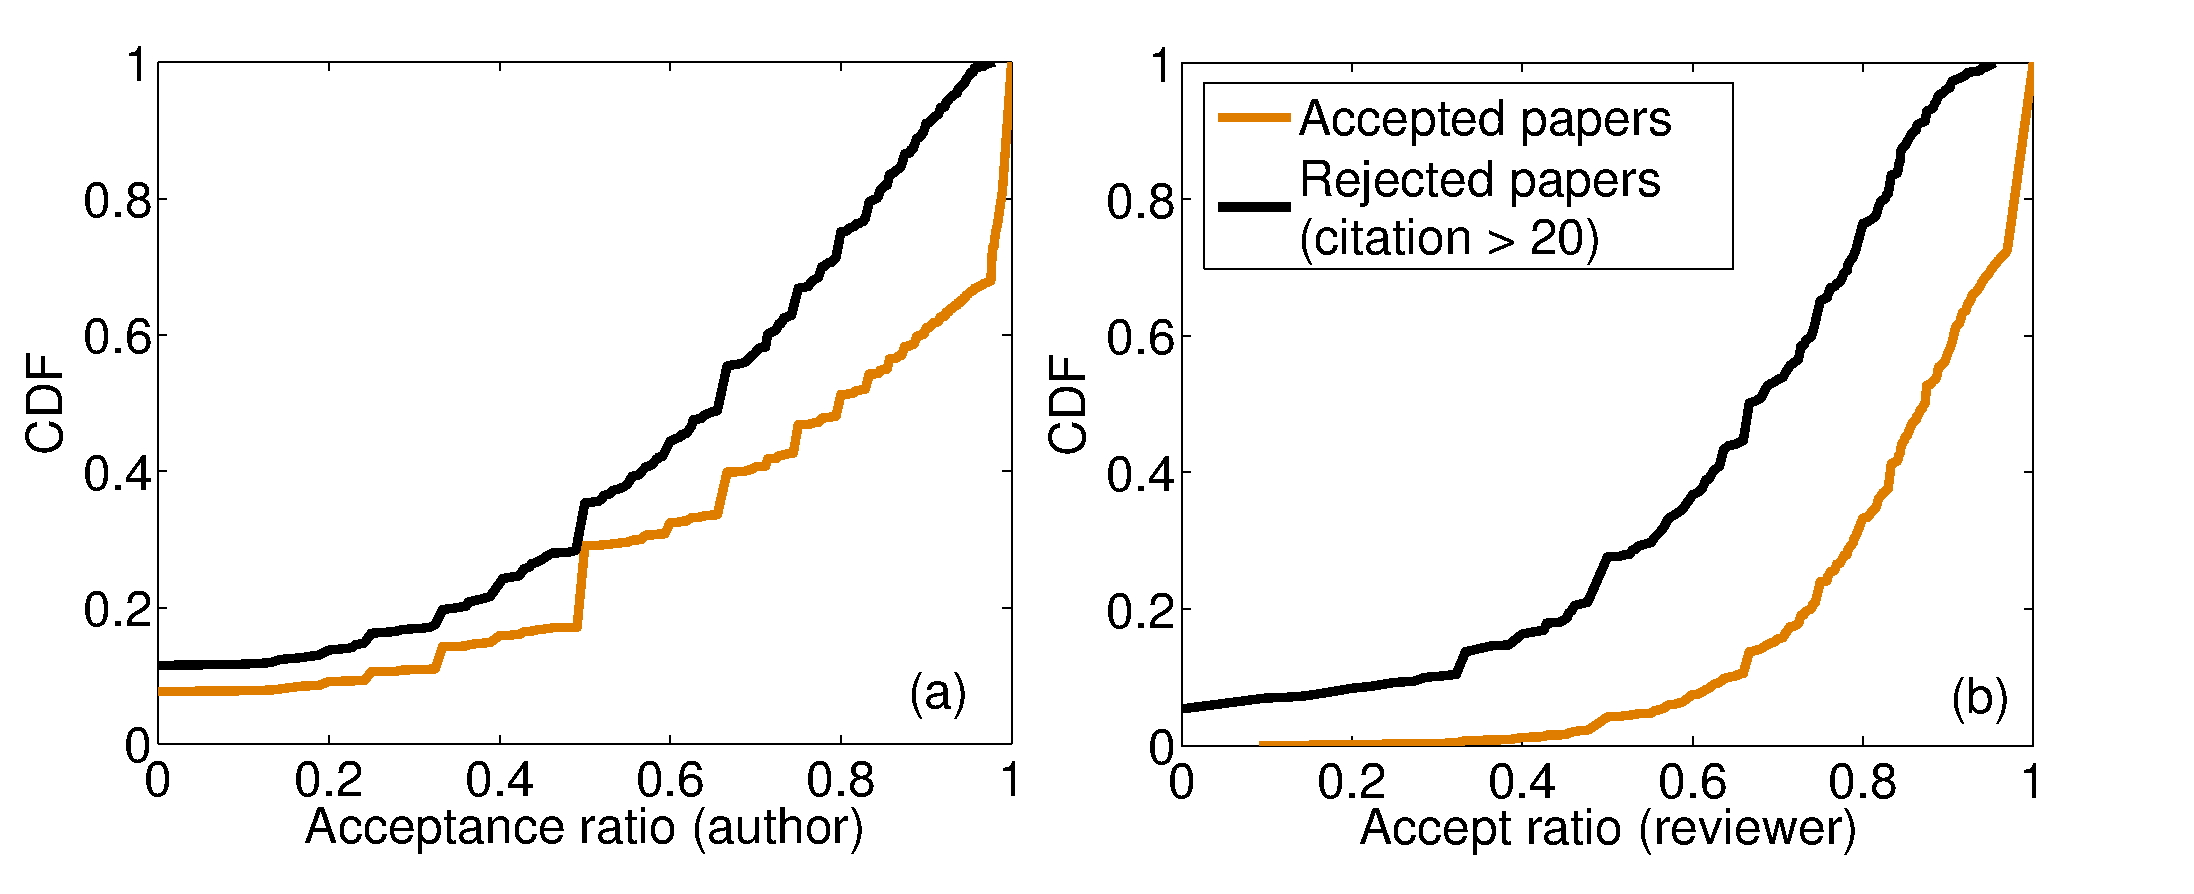
\includegraphics[scale=0.17]{./texfiles/Chapter_4/jcdl/figures/highly_cited_rejected-eps-converted-to.pdf}
\caption{CDF of (a) acceptance ratio of authors and (b) accept ratio of reviewers for accepted papers and highly cited rejected papers.}
\label{fig10}
\vspace{3mm}
\end{figure}

\begin{figure}
\centering
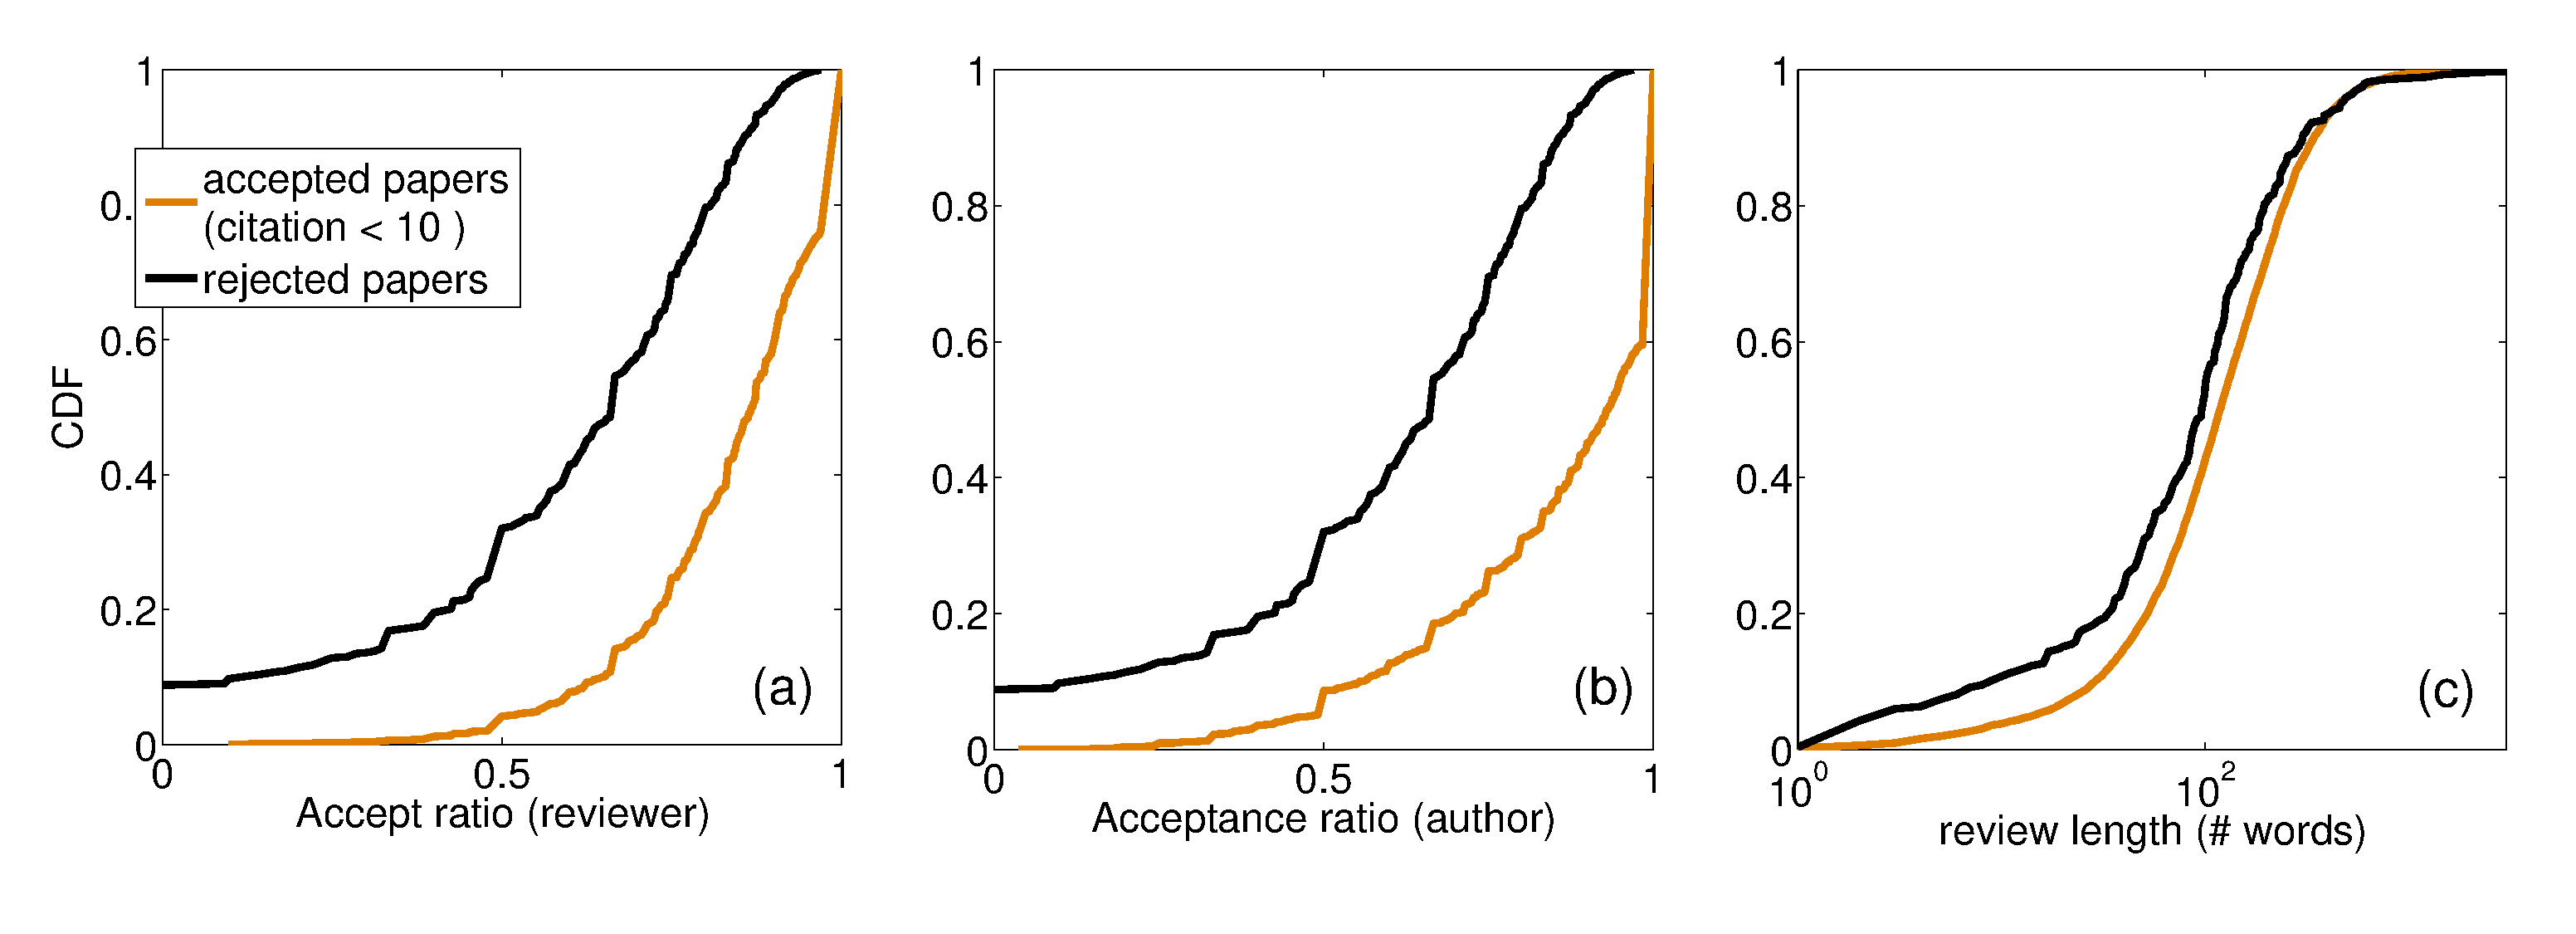
\includegraphics[scale=0.17]{./texfiles/Chapter_4/jcdl/figures/low_cited_accepted-eps-converted-to.pdf}
\caption{CDF of (a) accept ratio of reviewers, (b) acceptance ratio of authors (c) length of the review text (\# words) for rejected papers and low cited accepted papers.}
\label{fig11}
\vspace{3mm}
\end{figure}



\label{irregular_cases}

In this section we investigate in more detail the irregular cases, i.e., the highly cited rejected papers and the low cited accepted papers. Note that we only consider papers which were published before 2012 so that each paper gets at least three years of exposure to the scientific community for garnering citations.

\noindent{\em Highly cited rejected papers:} We previously observed that on average the accepted papers tend to be cited more often than the rejected ones. Nevertheless, we find several papers (call it the set $P$) which were rejected at JHEP but were able to acquire more citations after getting accepted elsewhere. We consider only those papers in $P$ that have at least 20 citations which is twice the average citation of the rejected papers.
Manually looking into some of the review text we observed that in several cases the reviewer found the topic of research to be interesting but out of JHEP's scope. On deeper investigation we found that acceptance ratio of the authors of these papers is lower than that of the authors of accepted papers (figure~\ref{fig10}(a)) indicating that author's reputation might have played a role in the rejection. We further observe that the accept ratio of the reviewers, these papers were assigned to, to be significantly less than that of the accepted papers (figure~\ref{fig10}(b)). This indicates that the papers got assigned to stricter reviewers and hence the rejection.

\noindent{\em Low cited accepted papers:} We now look into the complementary i.e., the papers which were accepted but failed to make impact on the scientific community and accrued very low citations (typically $< 10$). Ideally, these papers should have been rejected, hence we investigate how different these are in terms of author's acceptance ratio and reviewer's accept ratio. While the authors of these papers have higher acceptance ratio (figure~\ref{fig11}(a)), they were also assigned to reviewers who are less strict (figure~\ref{fig11}(b)). These observations indicate that either the contributing author's reputation might have played a role in their acceptance or were lucky to have been reviewed by lenient referees. Review report also seem to be sloppy in many cases with the reviewer not even mentioning the reason for acceptance. We also observe the length of the review report (in terms of the number of words) on average to be less than that of the rejected papers (figure~\ref{fig11}(c)). 
%\medskip